\subsection{Satteins}
Das Testgebiet des Systems war in Satteins. In den Folgenden Punkten wird kurz das Gebiet beschrieben und wie die Daten Erfasst wurden.
\subsubsection{Topologie}
Wie im linken Bild nachfolgend (\fref{bSatteins} (a)) zu sehen ist, wurden in Satteins sechs Geräte installiert. Jedes dieser Geräte wurde an den Ein- und Ausfahrtspunkte, sowie an strategisch interessanten Verkehrspunkten platziert. Mit diesen sechs Geräten ist es möglich den grössten Teil des Verkehrsflusses in Satteins quantitativ zu rekonstruieren. Mit Hilfe des rechten Bildes (\fref{bSatteins}(b)) wird jede Abzweigung welche die Verkehrsteilnehmer nehmen können identifiziert und in der Berechnung des Verkehrsflusses beachtet. Dabei werden die Geräte schematisch auf einen Knotenpunkt, bei den Ein- und Ausfahrtsstrassen gelegt und die zwei Anderen werden auf die Mitte der Straße projiziert. So löst sich der Verkehrsfluss im Graphen darstellen und zu Letzt auf die Karte von Satteins zurück projizieren.

\begin{figure}[H]
  \centering
  \subfigure[Satteins]{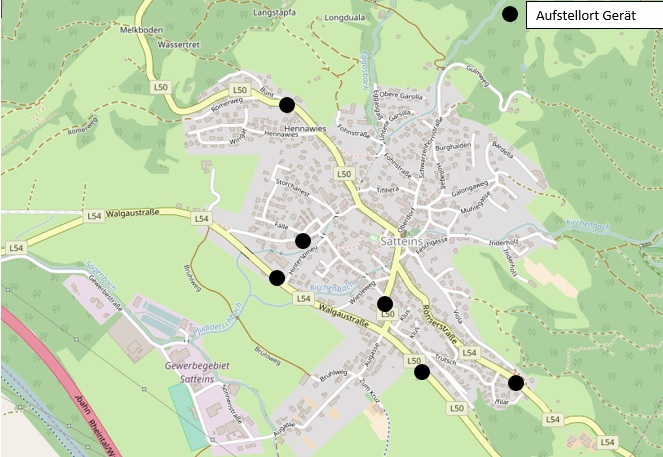
\includegraphics[width=0.5\textwidth]{Resultate/Satteins.jpg}}
  \subfigure[Graph von Satteins]{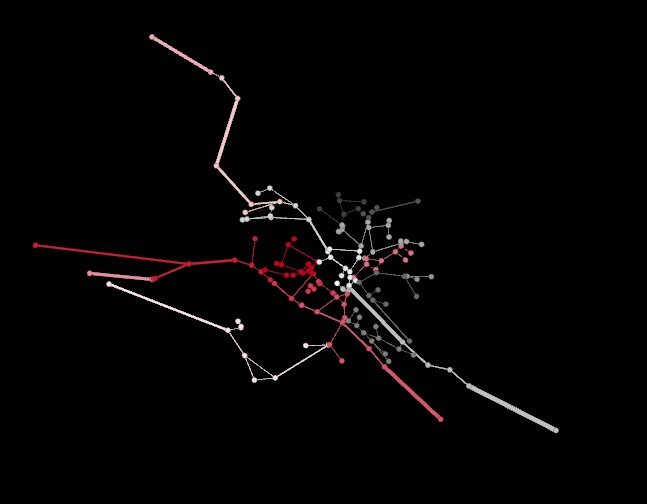
\includegraphics[width=0.44\textwidth]{Resultate/Topologie.jpg}}
  \caption{Topologie von Satteins}
  \label{bSatteins}
\end{figure}

\subsubsection{Erfassung der Daten}
Alle Daten welche die Geräte aufgezeichnet haben, wurden auf den internen SD-Karten abgespeichert und jeden zweiten Tag mittels Smartphone-Hotspot auf den Laptop übertragen. Dabei wurde bei jedem einzelnen Gerät der Feature Vektor, sowie der Temperaturverlauf heruntergeladen. Die Feature Vektoren der Geräte enthielten mehrere tausend Einträge mit vorbeifahrenden Verkehrsteilnehmern.